\documentclass[11pt,a4paper,BCOR12mm, headexclude, footexclude, twoside, openright]{scrartcl} 
\usepackage[scaled]{helvet}
\usepackage[british]{babel}
\usepackage[utf8]{inputenc}
\usepackage[T1]{fontenc}
\usepackage{fancyhdr}
\usepackage{lastpage}
\usepackage{ifthen}
\usepackage{amsmath,amsfonts,amsthm}
\usepackage{sfmath}
\usepackage{makecell}
\usepackage{booktabs}
\usepackage{sectsty}
\usepackage{graphicx}

%\KOMAoptions{optionenliste}
%\KOMAoptions{Option}{Werteliste}


\addtokomafont{caption}{\small}
%\setkomafont{descriptionlabel}{\normalfont
%	\bfseries}
\setkomafont{captionlabel}{\normalfont
	\bfseries}
\let\oldtabular\tabular
\renewcommand{\tabular}{\sffamily\oldtabular}
\KOMAoptions{abstract=true}
%\setkomafont{footnote}{\sffamily}
%\KOMAoptions{twoside=true}
%\KOMAoptions{headsepline=true}
%\KOMAoptions{footsepline=true}
\renewcommand\familydefault{\sfdefault}
\renewcommand{\arraystretch}{1.1}
\newcommand{\horrule}[1]{\rule{\linewidth}{#1}}
\setlength{\textheight}{230mm}
\allsectionsfont{ \normalfont\scshape}
\let\tmp\oddsidemargin
\let\oddsidemargin\evensidemargin
\let\evensidemargin\tmp
\reversemarginpar

\numberwithin{equation}{section} % Number equations within sections (i.e. 1.1, 1.2, 2.1, 2.2 instead of 1, 2, 3, 4)
\numberwithin{figure}{section} % Number figures within sections (i.e. 1.1, 1.2, 2.1, 2.2 instead of 1, 2, 3, 4)
\numberwithin{table}{section} % Number tables within sections (i.e. 1.1, 1.2, 2.1, 2.2 instead of 1, 2, 3, 4)

\setlength\parindent{0pt}


\begin{document}


%\sffamily

\fancypagestyle{plain}
{%
  \renewcommand{\headrulewidth}{0pt}%
  \renewcommand{\footrulewidth}{0.5pt}
  \fancyhf{}%
 \fancyhead[R]{\emph{\footnotesize \today}}
  \fancyfoot[C]{\emph{\footnotesize Boqi Chen, bochen@student.ethz.ch}\\ \emph{\footnotesize Xin Wu, xinwuxin@student.ethz.ch}}%
}



\titlehead
{
	ETH Zürich\\%
	D-ITET\\%
	Biomedical Engineering\hfill
    Master Studies%
}

\subject{\vspace{-1ex} \horrule{2pt}\\[0.15cm] {\textsc{\texttt{Biomedical Imaging}}}}

\title{Homework \#1 - Signals \& Systems\\[0.5cm]}

\author{\bfseries{Xin Wu \\ \textbf{Boqi Chen\\}}\vspace{-2ex}}
\date{\begin{tabular}{cc}
  \textsc{Date:}& \textsc{\emph{\today}}\\
  \textsc{Due :}& \textsc{\emph{28th September 2020}}\vspace{3ex}
\end{tabular}}

\maketitle

%--------------------------------------------
\newpage

\section{Plane waves} 
\subsection{Theory}

One way to visualize a wave is to display it's lines of equal phase. Usually we use the phase of peak or valley. For plane waves, the lines of equal phase are just a list of parallel lines:

\begin{equation}
    k_x x + k_y y = 2 \pi n, n \in \mathcal{Z}
\end{equation}

\begin{figure}[h!]
\centering
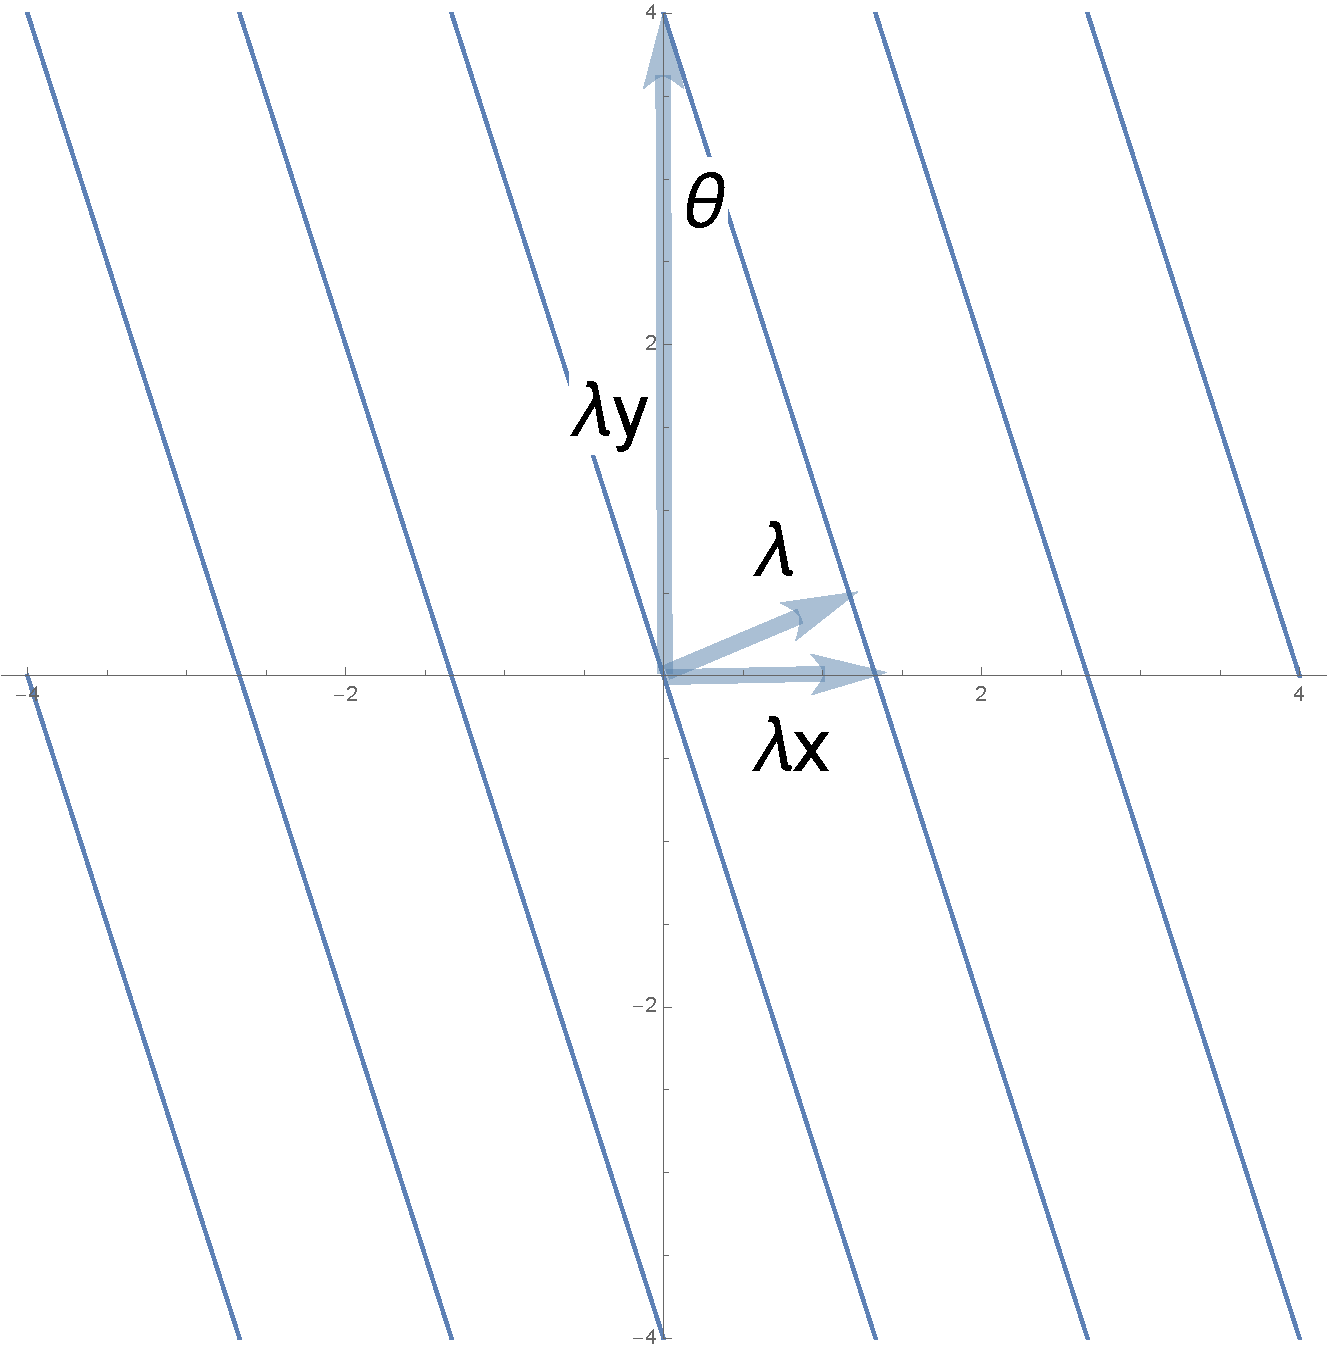
\includegraphics[scale=0.5]{Equal_Phase.pdf}
\caption{Lines of Equal Phase}
\end{figure}

This figure contains all the information we need to understand the properties of plane waves. First the direction:

\begin{equation}
\theta = arctan (\frac{k_y}{k_x})
\end{equation}
%-------------------------------

Or we can use the 2-D direction vector by calculating the gradient of phase:

\begin{equation}
    \nabla \phi = (k_x,k_y)
\end{equation}

The the wavelength:

\begin{equation}
    \lambda = \lambda_x cos(\theta) = \frac{2 \pi}{\sqrt{k_x ^2 + k_y ^2}}
\end{equation}

Last thing here: the function in this exercise is just the space component of a 2D plane wave, without the time component it's static and not propagating. 

\subsection{Coding Results}

For a selection of 
\begin{equation}
   k_x = 10, k_y = 10
\end{equation}

We have the following results:

\begin{figure}[h!]
\centering
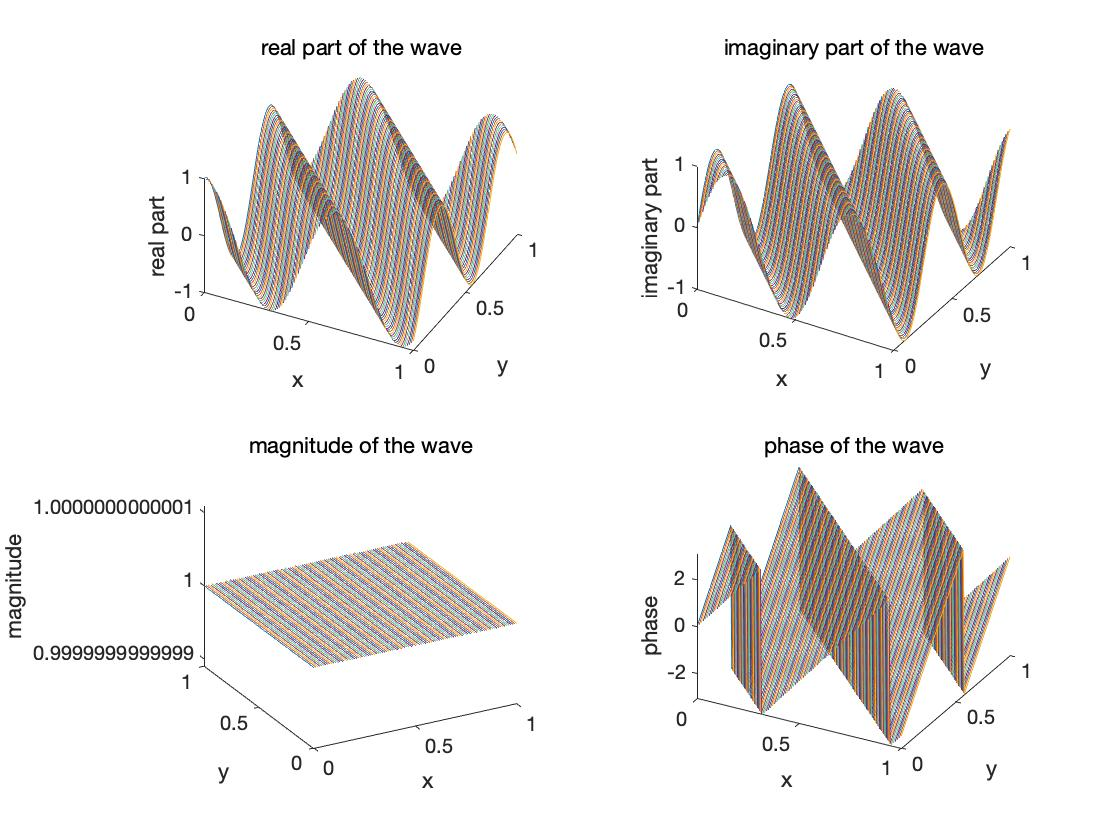
\includegraphics[scale=0.35]{wave2.jpg}
\caption{Real Part, Imaginary Part, Magnitude and Phase of the wave}
\end{figure}

\newpage

The LSI system applied to the wave is:

\begin{equation}
   S[f(x,y)] = \alpha f(x,y)
\end{equation}

where 
\begin{equation}
   \alpha = 2
\end{equation}

We have the following results:

\begin{figure}[h!]
\centering
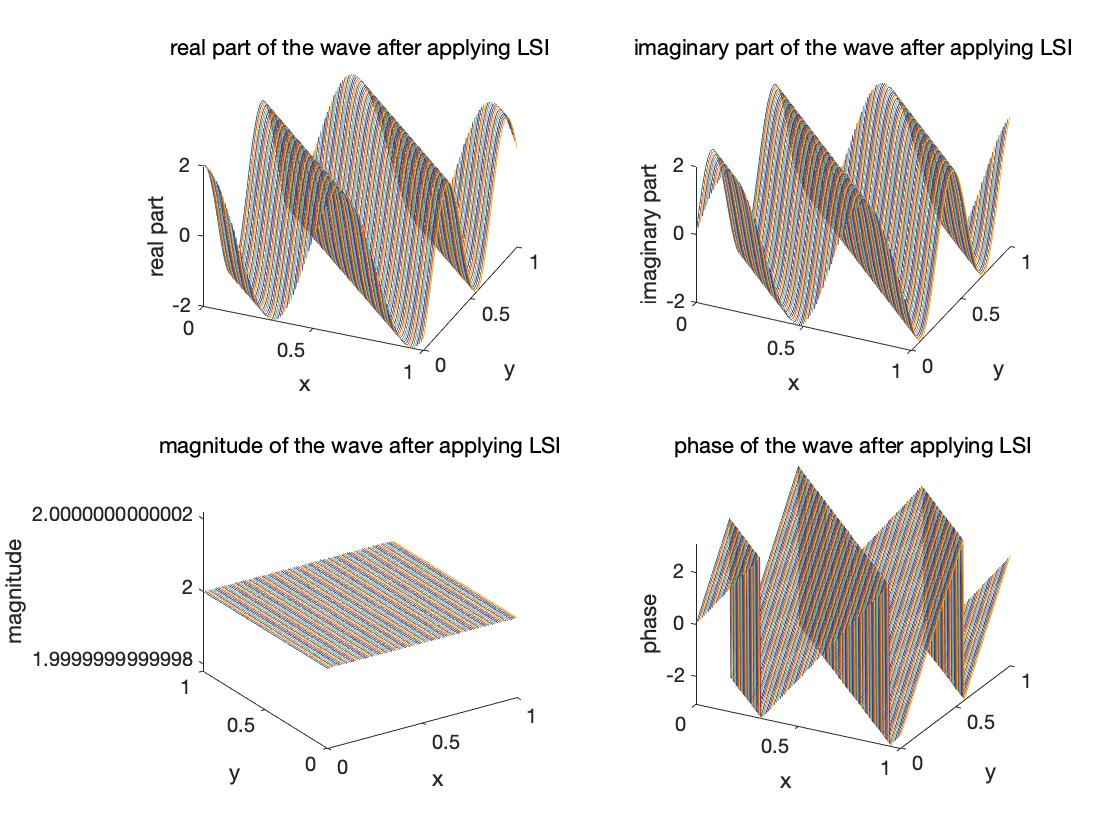
\includegraphics[scale=0.35]{wave3.jpg}
\caption{Real Part, Imaginary Part, Magnitude and Phase of the wave applied LSI}
\end{figure}

\newpage
\section{Fast Fourier Transform (FFT)}

The formula for DFT is:

\begin{equation}
    \mathcal{F}[f](k_m) = exp(-i k x_0) \sum_{n=0}^{N-1} f(x_n) exp(-\frac{2 \pi m n}{N})
\end{equation}

So the sum part is called DFT. We still need a constant phase correction $exp(-i k x_0) $ to get the real fourier transform. That's the key point in this exercise.


\subsection{Directly using FFT}

The FFT always assumes the starting point of a signal sequence to be on the very left. By directly using FFT in MATLAB, what we can get is actually a frequency sequence starting from k=0. Also because the Fourier Transform is periodic (as the original signal is discrete), we get another peak on the very right. Thus in the first picture we have a $Sinc(x)$ function divided in to two halves.

\begin{figure}[h!]
\centering
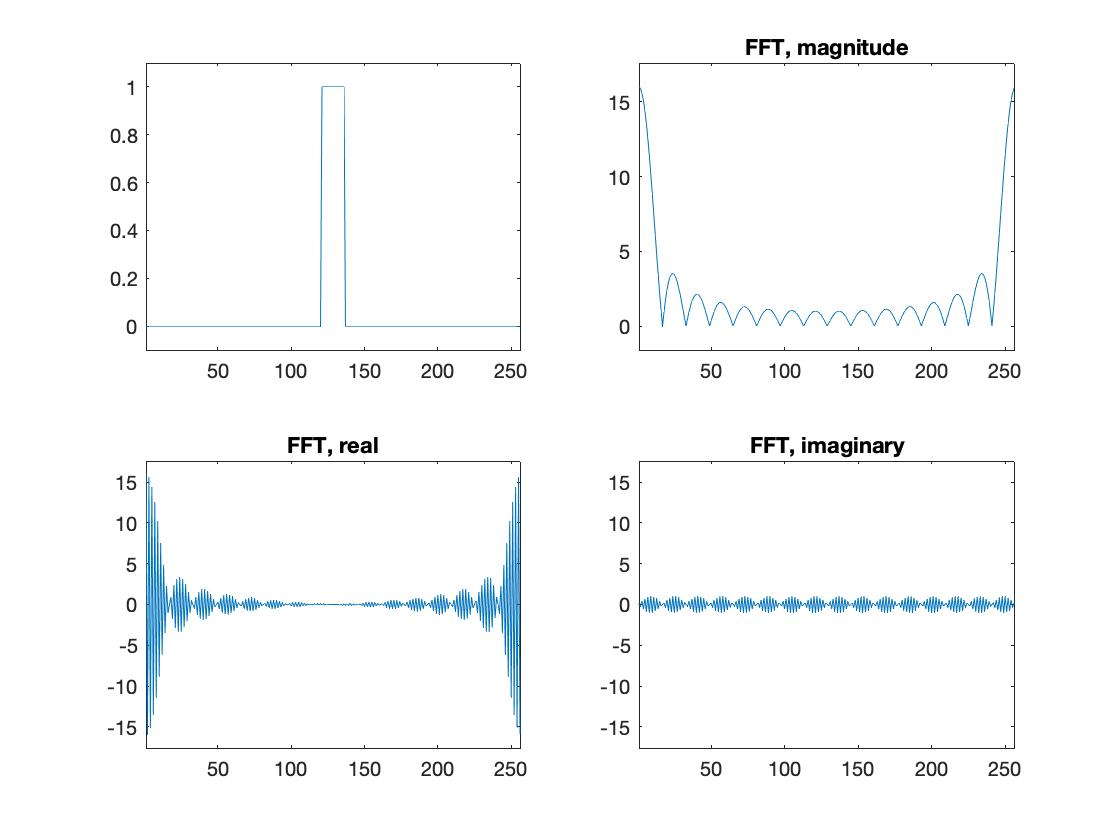
\includegraphics[scale=0.35]{2-1.jpg}
\caption{Directly Using FFT}
\end{figure}

\newpage
\subsection{Using FFTShift}

By applying FFTShift, the frequency sequence is now
correctly ordered. However, the Rectangular in original signal is not centered about zero, resulting in a linearly-increasing phase shift of the FFT output, which adds a high frequency oscillation. This can be explained time-shifted Fourier Transform Theorem:

\begin{equation}
    \mathcal{F}[f(x-a)] = exp(-i k a) F(k)
\end{equation}
\begin{figure}[h!]
\centering
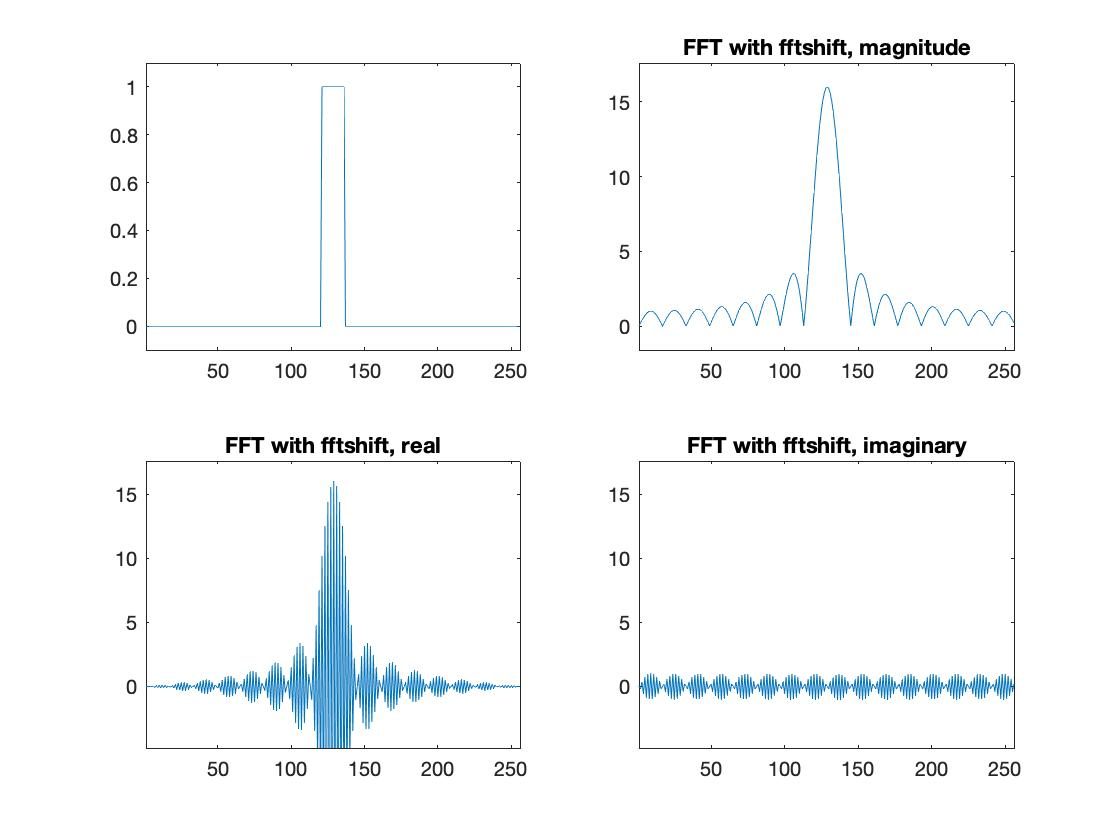
\includegraphics[scale=0.35]{2-2.jpg}
\caption{Using FFTShift}
\end{figure}

\newpage

\subsection{Add Phase Correction}

Both examples above have high frequency oscillating components over Sinc function. This, as mentioned before, can be compensated by manually adding the phase correction part:

\begin{equation}
    corr(k) = exp(-i k x_0) 
\end{equation}

For 2-D cases is:

\begin{equation}
    corr(k) = exp(-i (k_x x_0 + k_y y_0)) 
\end{equation}

\begin{figure}[h!]
\centering
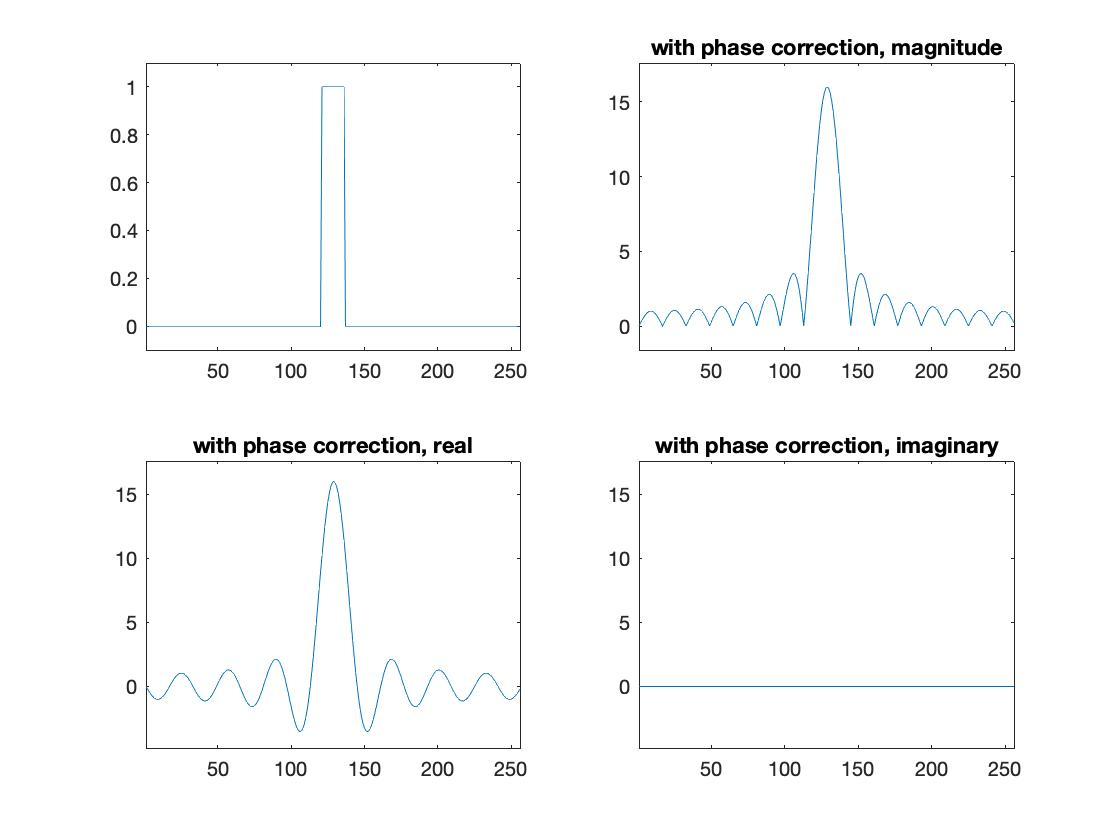
\includegraphics[scale=0.35]{2-3.jpg}
\caption{Adding Phase Correction}
\end{figure}

Now the high frequency oscillating parts disappear.
\newpage
\subsection{Shifting the Original Signal}

Instead of shifting the frequency sequence, we can shift the original signal sequence before FFT:

\begin{equation}
    fft \_ rect=fftshift(fft(fftshift(rect)));
\end{equation}

However, in this case, the centering point of the original signal sequence is not indexed by an integer. Because the FFTShift can only shift an array around, it cannot cope with points indexed by non-integer numbers. So the original signal after shifting is slightly unsymmetrical. Thus there exists an imaginary part resulting small high frequency oscillating. 

\begin{figure}[h!]
\centering
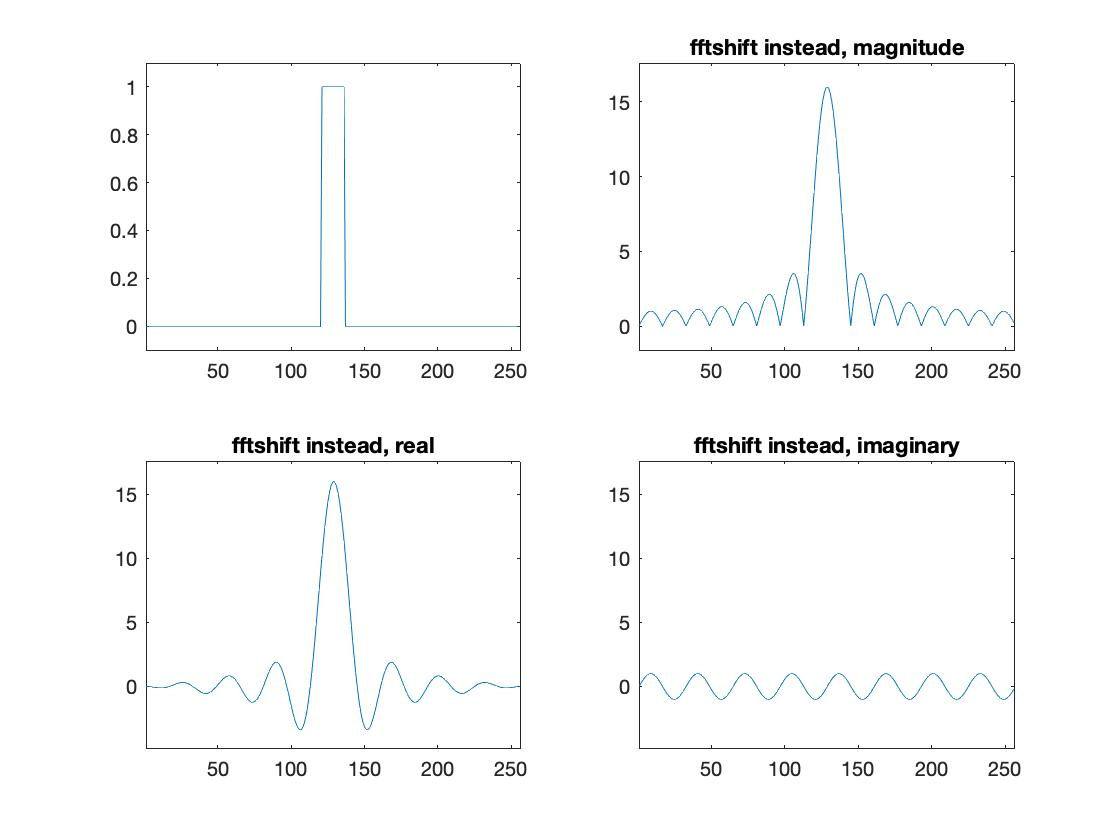
\includegraphics[scale=0.35]{2-4.jpg}
\caption{Shifting the Original Signal}
\end{figure}




\newpage



\section{Building a Comb}
\subsection{Theory}

The definition of Dirac's Comb function is:

\begin{equation}
    Comb(x) = \sum_{n} \delta(x - n \Delta x)
\end{equation}

As a periodical function, it can always be expanded into Fourier Series:

\begin{equation}
    Comb(x) = \frac{1}{\Delta x} \sum_{n} exp(i \frac{2 \pi n x}{\Delta x})
\end{equation}

The Fourier Transform of a single exponential function is a single Dirac function:

\begin{equation}
\mathcal{F}[exp(i k_0 x)] = \delta (k - k_0)
\end{equation}

So the can easily derive the Fourier Transform of Dirac's Comb function:

\begin{equation}
    \mathcal{F} [Comb(x)] = \frac{1}{\Delta x} \delta (k - n \frac{2 \pi }{\Delta x}) = \frac{1}{\Delta x} \delta (k - n \Delta k)
\end{equation}

We have:

\begin{equation}
    \Delta k = \frac{2 \pi}{ \Delta x}
\end{equation}

That's the essence of this exercise: if you have larger $\Delta x$, you'll have smaller $\Delta k$, vice versa.

\newpage
\subsection{Coding Results}

\subsubsection{Adding Impulse}

When adding impulses, the more impulses are added, the more resemble the FFT of the comb function is to itself. 

\begin{figure}[h!]
\centering
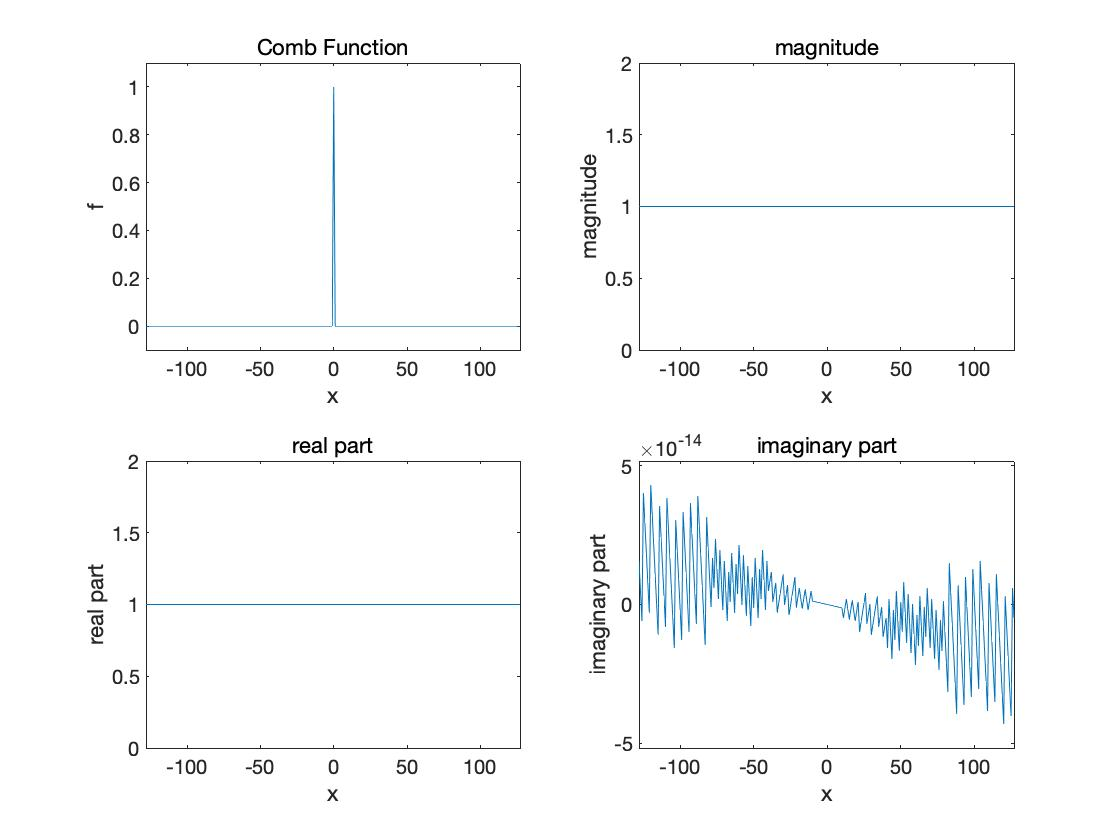
\includegraphics[scale=0.35]{1.jpg}
\caption{Single Impulse}
\end{figure}

\newpage

\begin{figure}[h!]
\centering
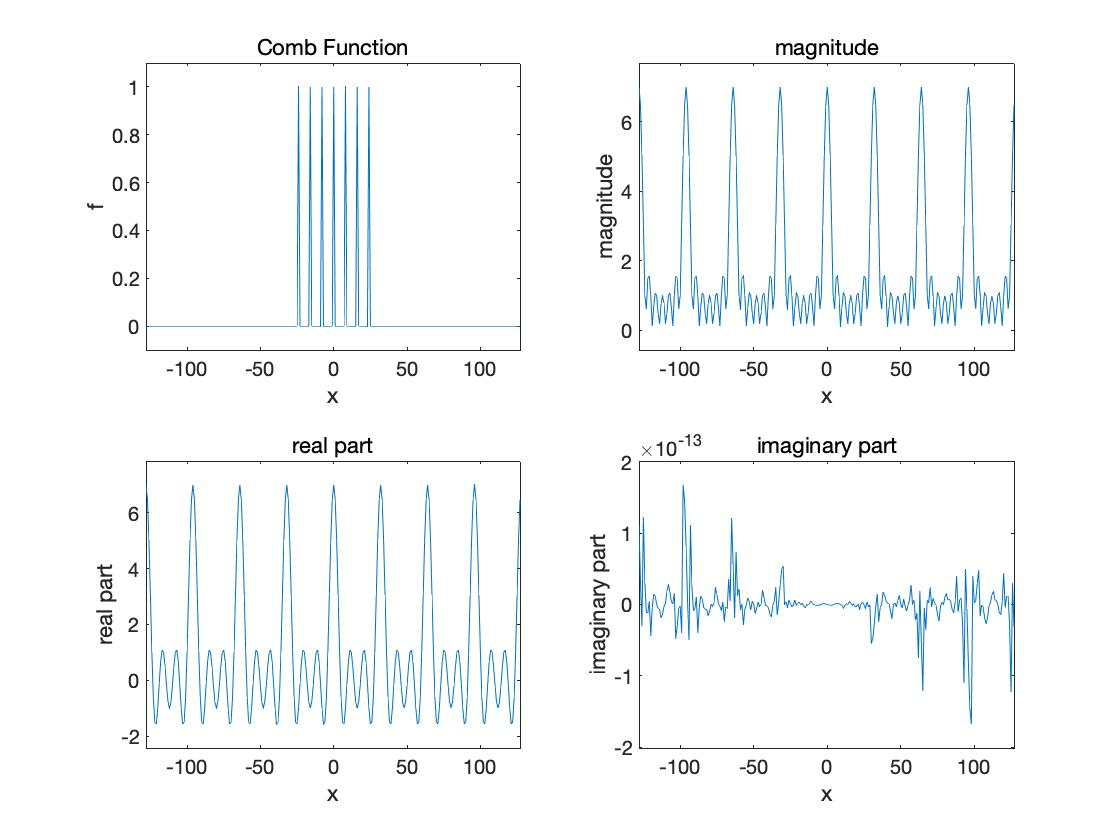
\includegraphics[scale=0.35]{2.jpg}
\caption{Seven Impulses}
\end{figure}

\newpage

\begin{figure}[h!]
\centering
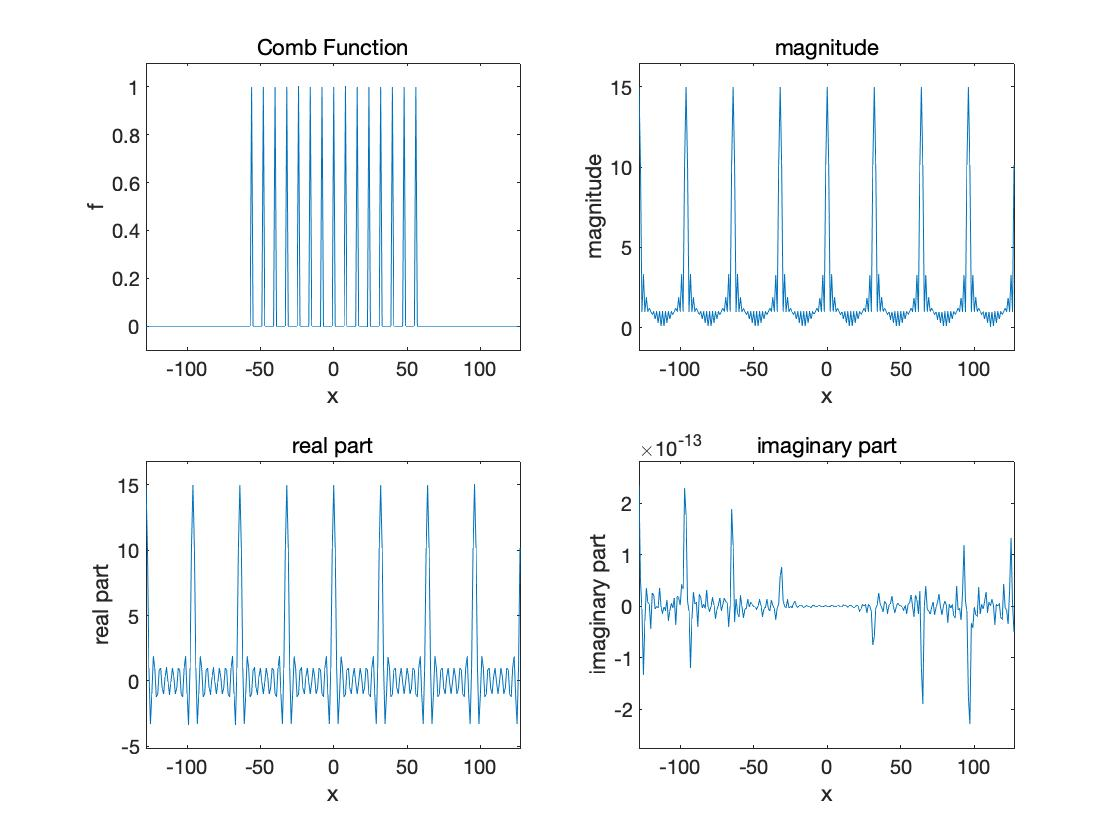
\includegraphics[scale=0.35]{8.jpg}
\caption{Fifteen Impulses}
\end{figure}

\newpage

\begin{figure}[h!]
\centering
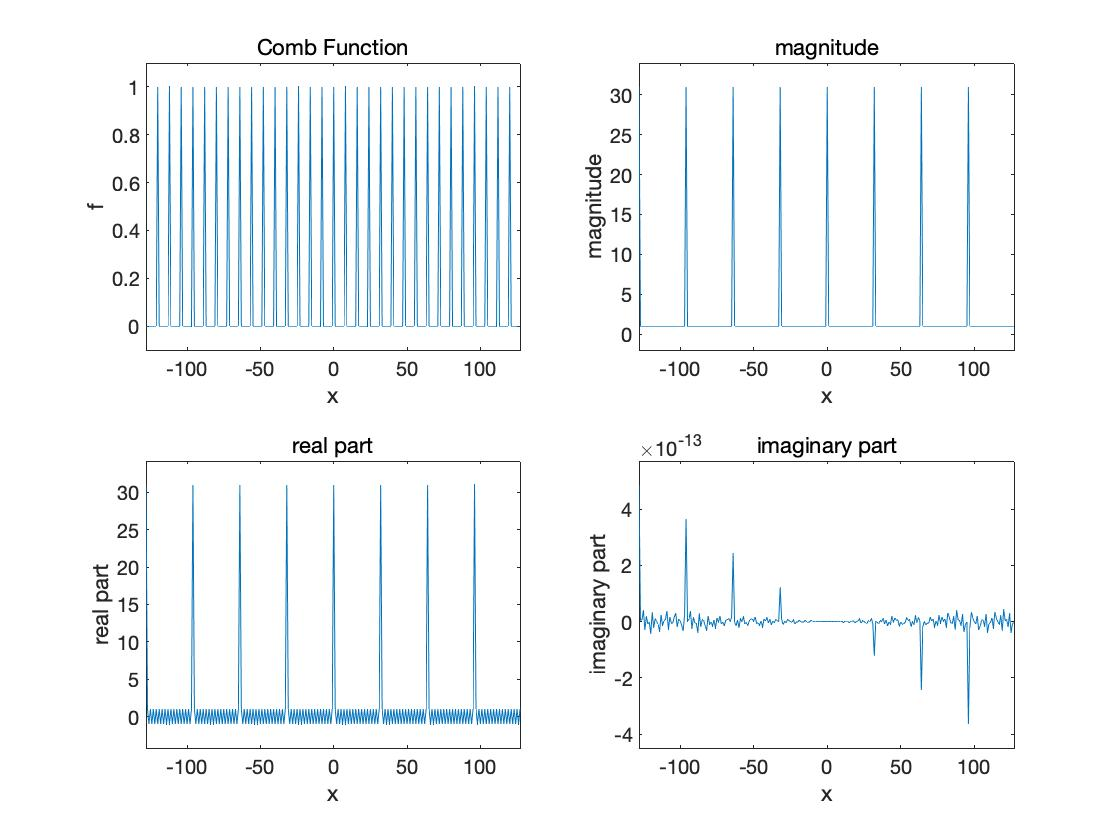
\includegraphics[scale=0.35]{16.jpg}
\caption{Thirty-one Impulses}
\end{figure}

\newpage

\newpage

\subsection{Varying $\Delta$ x}

From the figures below, we can easily visualize the relationship:
\begin{equation}
    \Delta k = \frac{2 \pi}{ \Delta x}
\end{equation}

As $\Delta x$ increases, the $\Delta k$ just decreases. which is indicated by the equation 3.6.

\begin{figure}[h!]
\centering
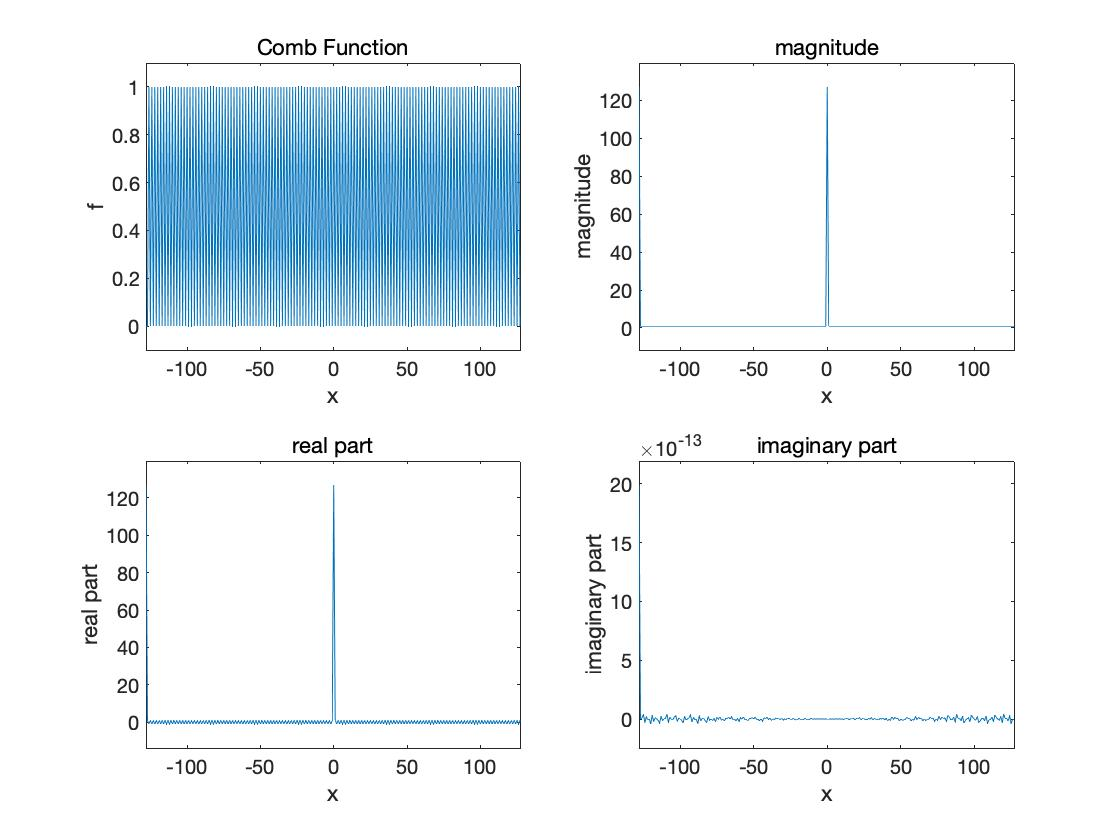
\includegraphics[scale=0.35]{d2.jpg}
\caption{$\Delta$ x = 2}
\end{figure}

\newpage

\begin{figure}[h!]
\centering
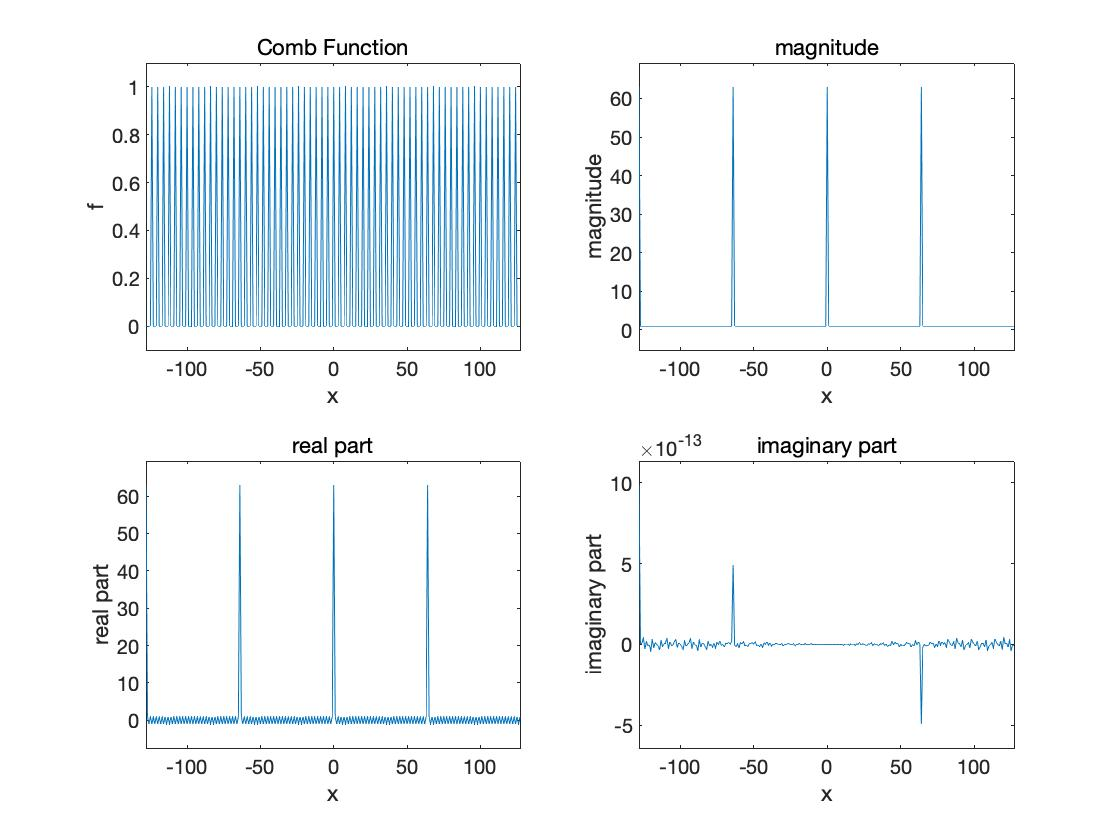
\includegraphics[scale=0.35]{d4.jpg}
\caption{$\Delta$ x = 4}
\end{figure}


\newpage


\begin{figure}[h!]
\centering
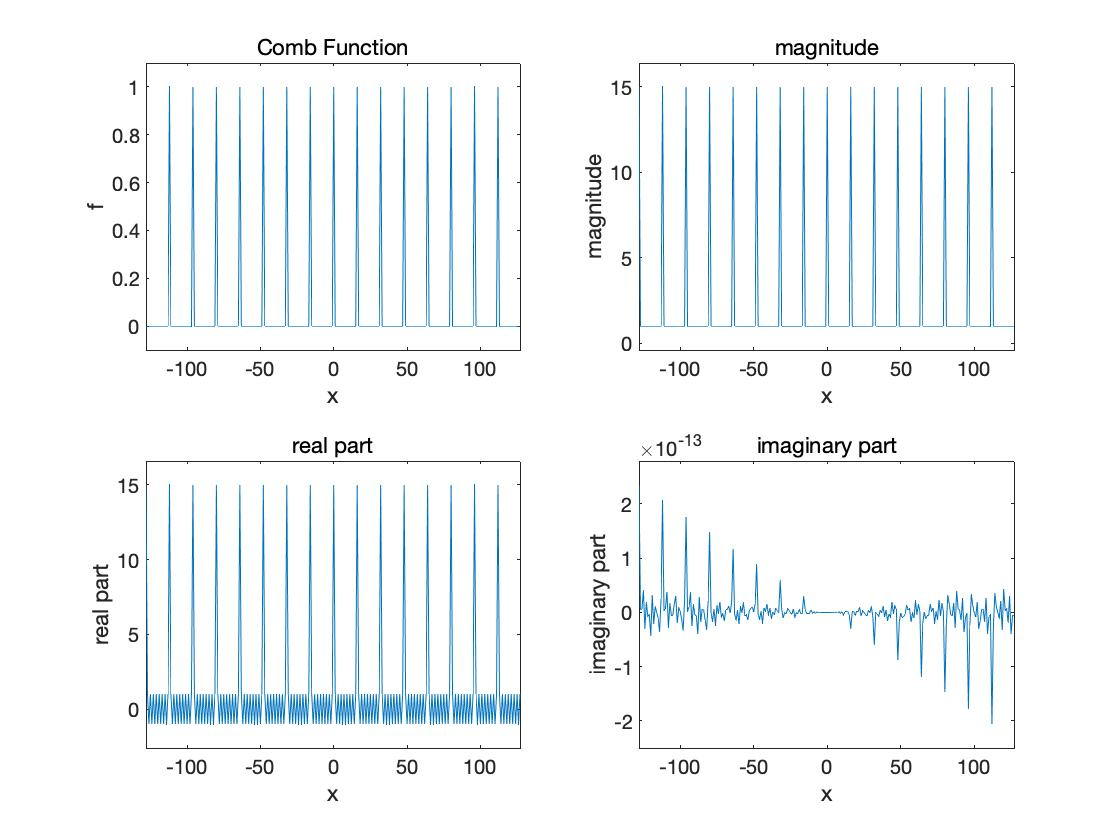
\includegraphics[scale=0.35]{d16.jpg}
\caption{$\Delta$ x = 16}
\end{figure}

\newpage

\begin{figure}[h!]
\centering
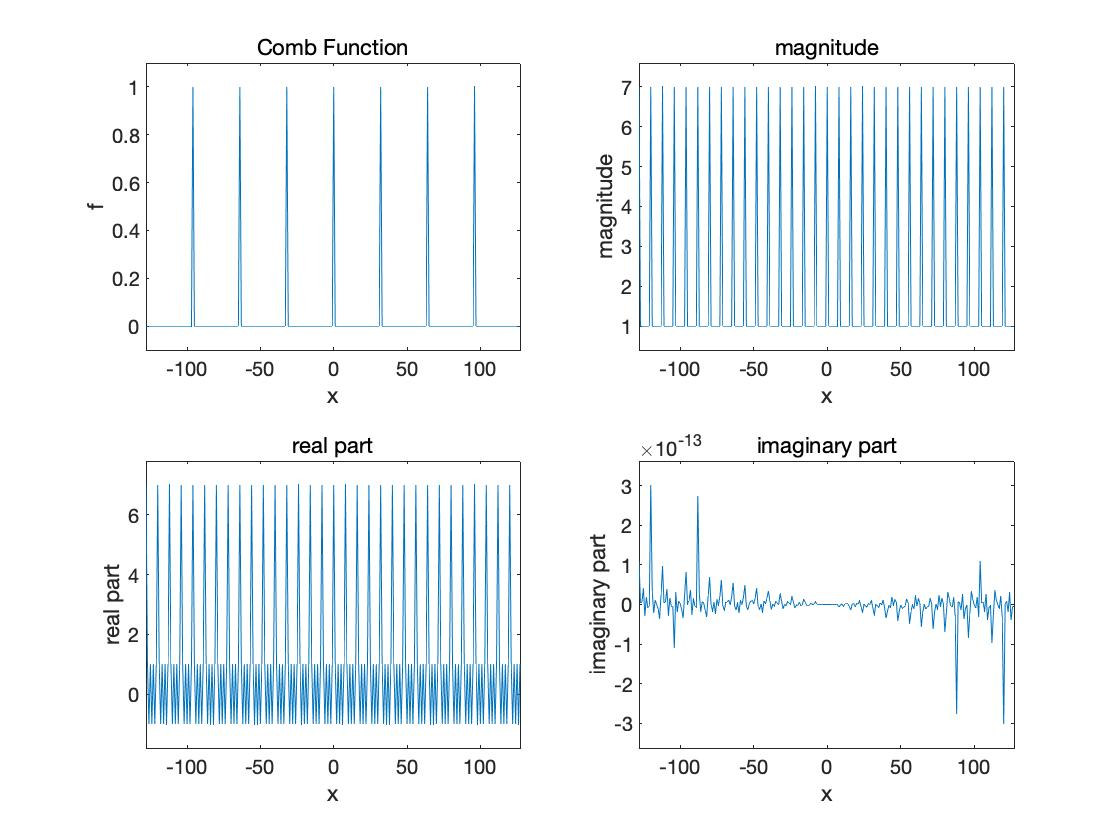
\includegraphics[scale=0.35]{d32.jpg}
\caption{$\Delta$ x = 32}
\end{figure}

\end{document}


\subsubsection{Varying $\Delta x$}

\end{document}

\end{document}